\documentclass[hidelinks]{ctexart}

\usepackage{van-de-la-illinoise}

\begin{document}

\section{电子的自旋和原子能级的精细结构} % (fold)
\label{sec:电子的自旋和原子能级的精细结构}

\begin{figure}[ht]
    \centering
    \incfig{6cm}{LQuantum}
    \caption{角动量量子化}
\end{figure}
\vspace{-\baselineskip}
\begin{align*}
    L &= \sqrt{l\pare{l+1}}\hbar, \\
    L_z &= m\hbar,\quad m_l = 0,\pm 1,\pm 2,\cdots,\pm l.
\end{align*}

\subsection{轨道磁矩} % (fold)
\label{sub:轨道磁矩}

\subsubsection{原子轨道磁矩} % (fold)
\label{ssub:原子轨道磁矩}

闭合轨道电子运动产生磁偶极矩, $\+v\mu_l = IS\+vn$,
\[ \resumath{\+v\mu_l = -\frac{e}{2m_e}\+vL.} \]
考虑到角动量量子化,
\begin{align*}
    \mu_l &= \frac{e}{2m_e}\sqrt{l\pare{l+1}}\hbar = \sqrt{l\pare{l+1}}\mu_B. \\
    \mu_{lz} &= -\frac{e}{2m_e}m_l\hbar = -m_l\mu_B.\\
\end{align*}
其中
\[ \resumath{\mu_B = \frac{e\hbar}{2m_e}} \approx \SI{9.274e-24}{\joule\per\tesla} \approx \SI{5.788e-5}{\eV\per\tesla} \]
谓\gloss{Bohr磁子}. 电子轨道回磁比谓
\[ \frac{\abs{\mu_{lz}}}{L_z} = \frac{e}{2m_e}. \]

% subsubsection 原子轨道磁矩 (end)

\subsubsection{磁矩与磁场相互作用} % (fold)
\label{ssub:磁矩与磁场相互作用}

磁矩$\+v\mu$在磁场$\+vB$中有取向势和受力
\[ U = -\+v\mu\cdot \+vB,\quad \+vF = -\grad U = -\+v\mu\+v\cdot\grad \+vB. \]
如果磁场均匀, 则磁矩受力为零. 所受力矩为
\[ \+v\tau = \+v\mu\times \+vB = \+dtd{\+vL} = \+v\mu\times \+vB. \]
原子中电子轨道磁矩
\[ \tau = \+dtd{\+vL} = \+v\mu_l\times \+vB = -\frac{e}{2m_e}\+vL\times \+vB = \+v\omega \times \+vL, \]
其中
\[ \+v\omega = \frac{e}{2m_e}\+vB = \frac{\mu_B}{\hbar}\+vB. \]
均匀磁场中角动量$\+vL$绕$\+vB$以频率$\omega$做Larmor进动.

% subsubsection 磁矩与磁场相互作用 (end)

\subsubsection{Stern-Gerlach实验} % (fold)
\label{ssub:stern_gerlach实验}

\begin{figure}[ht]
    \centering
    \includegraphics[width=10cm]{src/SternGerlach.png}
    \caption{Stern-Gerlach实验装置}
\end{figure}
由原子炉喷出的原子束经过扁平狭缝准直后经过磁场区, $\displaystyle \+DzD{\+vB}\neq 0$, 将导致原子受力非零. 若在某处有
\[ \+DxD{B_z} = 0,\quad \+DyD{B_z} = 0, \]
则原子束仅受到$\+uz$方向的力, $\displaystyle F_z = \mu_{lz}\+DzD{B_z}$. 经典结果为$\mu_{lz} = \brac{-\mu_{l},+\mu_{l}}$. 考虑空间量子化, 则
\[ \mu_{lz} = -\frac{e}{2m_e}m_l \hbar = -m_l \hbar_B,\quad m_l = -l,-\pare{l-1}, \cdots, \pare{l-1}, l. \]
这意味着偏转也是量子化的.
\par
原子束应当分离为$2l+1$条, 且$l=0$处(不偏转)应当存在原子束. 且基态氢原子应当有$l=0$, 不应当发生偏转. 然而对氢原子的实验也发生了偏转.
\par
原子光谱还存在精细结构, Balmer线有若干条分立谱线. 且当原子放入外磁场中时, 会出现多条分裂谱, 发生Zeeman分裂.

% subsubsection stern_gerlach实验 (end)

\subsubsection{电子自旋} % (fold)
\label{ssub:电子自旋}

原子中的电子除了围绕原子核的轨道运动外, 还有自旋运动.
\[ \+vS^2 = s\pare{s+1}\hbar^2,\quad S_z = m_s \hbar. \]
从氢原子束分裂结果可得$2s+1 = 2$, 从而
\[ s = \half \Rightarrow \abs{\+vS} = \frac{\sqrt{3}}{2}\hbar,\quad m_s = \pm \half \Rightarrow S_z = \pm \frac{\hbar}{2}. \]
从而电子自旋回磁比
\[ \frac{\abs{\mu_{sz}}}{S_z} = \frac{\mu_B}{\hbar/2} = \frac{e}{m_e}. \]
电子自旋磁矩
\begin{resume}
    \vspace{-\baselineskip}
\begin{align*}
    \+v\mu_s &= -\frac{e}{m_e}\+vS = -g_s\frac{\mu_B}{\hbar}\+vS,\\
    \mu_{sz} &= -\frac{e}{m_e}S_z = -g_s m_s \mu_B.
\end{align*}
\end{resume}
其中$g_s = 2$谓Land\'e $g$因子. 电子轨道磁矩
\begin{align*}
    \+v\mu_l &= -\frac{e}{2m_e}\+vL = -g_l \frac{\mu_B}{\hbar}\+vL, \\
    \mu_{lz} &= -\frac{e}{2m_e}L_z = -g_lm_l\mu_B.
\end{align*}
其中$g_l$谓轨道$g$因子, $g_l = 1$.

\begin{ex}
    电子经典半径$\displaystyle r_e = \frac{e^2}{4\pi \epsilon_0 m_e c^2} = \SI{2.8}{\femto\meter}$. 电子陀螺的角动量
    \begin{align*}
        & \int_0^{r_e} = \rho\pare{4\pi r^2}\,\rd{r}\cdot r\omega r = \frac{3}{5}m_e \omega r_e^2 = \frac{\hbar}{2}. \\
        & \Rightarrow v = \omega r_e \sim \SI{3.5e10}{\meter\per\second} \gg c.
    \end{align*}
\end{ex}

引入Dirac方程
\[ \pare{-i\hbar c\+v\alpha\+v\cdot\grad + V\pare{\+vr} + m_ec^2\alpha_0}\psi\pare{\+vr} = E\psi\pare{\+vr}, \]
可得电子具有自旋这一额外自由度, 自旋量子数$s=1/2$, 为电子内禀属性, 无经典对应.

\begin{sample}
    \begin{ex}
        设银原子从$T = \SI{1000}{\kelvin}$的加热炉内射出, 通过磁铁, 磁铁区长度$\SI{3.5}{\centi\meter}$, 磁场梯度$\SI{10}{\tesla\per\centi\meter}$, 求每束偏离量.
    \end{ex}
    \begin{solution}
        $\displaystyle F_z = -g_s \mu_b m_s \+DzD{B_z} \Rightarrow F_z = \pm \mu_0 \+DzD{B_z}$, 初始动能
        \[ \half Mv_x^2 = \frac{3}{2}kT \Rightarrow v_x = \sqrt{\frac{3k_BT}{M}}. \]
        穿越磁场的时间为
        \[ t = \frac{l}{v_x} = l\sqrt{\frac{M}{3k_BT}}, \]
        可得磁场出口处的偏移量
        \[ \Delta z = \half at^2 = \half \frac{F_z}{M}l^2 \frac{M}{3k_BT} = \pm \+DzD{B_z}\frac{\mu_B l^2}{6k_BT} = \SI{1.4e-4}{\meter}. \qedhere \]
    \end{solution}
\end{sample}

% subsubsection 电子自旋 (end)

% subsection 轨道磁矩 (end)

\subsection{自旋-轨道相互作用} % (fold)
\label{sub:自旋_轨道相互作用}

\subsubsection{自旋-轨道相互作用} % (fold)
\label{ssub:自旋_轨道相互作用}

电子的轨道运动会在原子内部产生一内磁场, 引入自旋后电子具有的内禀自旋磁矩与原子内磁场的磁相互作用会引起能量改变, 并产生能级分裂. 
\par
电子的轨道运动会在原子内部产生一个内磁场, 引入自旋后电阻具有的内禀自旋磁矩与原子内磁场的磁相互作用会引起相互作用能量的改变, 引发能级分裂.
\begin{align*}
    \+vB_e &= \rec{4\pi\epsilon_0 c^2} \frac{\+vj\times \+vr}{r^3} = \rec{4\pi\epsilon_0 c^2} \frac{Ze\pare{-\+vv}\times \+vr}{r^3} \\
    &= \frac{Ze}{4\pi\epsilon_0 m_e c^2r^3} \+vL.
\end{align*}
电子自旋磁矩在该磁场中具有取向是能
\[ U = -\+v\mu_s\cdot \+vB_e. \]
从而
\[ U = \rec{m_e^2c^2}\frac{Ze^2}{4\pi\epsilon_0 r^3}\+vS\cdot \+vL. \]
这是在相对于电子静止的坐标系中导出的, 需要变换到实验室坐标系. 由考虑Thomas旋进, 有
\begin{resume}
\vspace{-\baselineskip}
\begin{align*}
    \xi &= \rec{2m_e^2 c^2}\frac{Ze^2}{4\pi\epsilon_0 r^3}, \\
    U &= \xi \+vS\cdot \+vL.
\end{align*}
\end{resume}

\paragraph{定性解释原子光谱的精细结构} % (fold)
\label{par:定性解释原子光谱的精细结构}

由于自旋-轨道相互作用能的存在, $l\neq 0$的态会发生分裂.
\begin{sample}
    \begin{ex}
        估计氢原子的$\ce{2p}$态的自旋-轨道相互作用能和内磁场.
        \begin{align*}
            U &\approx \rec{2m_e^2 c^2}\frac{Ze^2}{4\pi\epsilon_0 r^3} \approx \SI{e-5}{\eV},\\
            U &= -\+v\mu_s \cdot \+vB_e = \abs{U}/\mu\+_B_ \approx \SI{0.2}{\tesla}.
        \end{align*}
    \end{ex}
\end{sample}

% paragraph 定性解释原子光谱的精细结构 (end)

% subsubsection 自旋_轨道相互作用 (end)

\subsubsection{总角动量} % (fold)
\label{ssub:总角动量}

电子的自旋磁矩在轨道运动产生的内磁场$\+vB_e$中将受到一个力矩的作用, 导致自旋角动量$\+vS$随时间改变, 不再守恒. 引入$\+vJ = \+vL+\+vS$, 并设$\+vJ^2 = j\pare{j+1}\hbar^2$, $J_z = m_j \hbar$, 则
\[ \begin{cases}
    \displaystyle \+dtd{\+vS} = \xi\pare{r} \+vL\times \+vS = \xi\pare{r} \+vJ\times \+vS, \\[.5em]
    \displaystyle \+dtd{\+vL} = \xi\pare{r}\+vS\times \+vL = \xi\pare{r} \+vJ\times \+vL.
\end{cases} \]
因此$\+vS$和$\+vL$以同样的角速度围绕$\+vJ$做Larmor进动.
\par
$\+vL^2$和$\+vS^2$仍然为守恒量, 故$l$和$s$是好量子数. $L_z$和$S_z$不是守恒量, 故$m_l$和$m_s$不是好量子数. $\+vJ^2$和$J_z$是守恒量, 故$j$和$m_j$是好量子数.

\paragraph{角动量相加的一般法则} % (fold)
\label{par:角动量相加的一般法则}

设$\+vJ_1$和$\+vJ_2$是体系的两个角动量,
\begin{align*}
    \+vJ_i^2 &= j_i\pare{j_i + 1}\hbar^2,\\
    J_{iz} &= m_{j_i} \hbar,\\
    m_{j_i} &\in \brac{-j_i,\cdots,j_i}.
\end{align*}
如果$\+vJ_1$和$\+vJ_2$无耦合, 则用量子数$\pare{j_1,m_1,j_2,m_2}$描述体系状态. 当$j_1$和$j_2$给定, 共有$\pare{2j_1+1}\pare{2j_2+1}$个状态.
\par
在有耦合的状态下, 总角动量量子数$j$的可能取值满足
\[ J_z = J_{1z} + J_{2z} \Rightarrow m = m_1 + m_2 \Rightarrow \abs{m}\+_max_ = j_1 + j_2 \Rightarrow j\+_max_ = j_1 + j_2. \]
从而
\[ j = j_1+j_2,\cdots, \abs{j_1 - j_2}. \]

% paragraph 角动量相加的一般法则 (end)

% subsubsection 总角动量 (end)

\subsubsection{角动量相加} % (fold)
\label{ssub:角动量相加}

将上述结论应用到$\+vL$和$\+vS$, 有
\[ j = l+s,\cdots,\abs{l-s}. \]
从而
\[ j = l+\half, \abs{l-\half}. \]

% subsubsection 角动量相加 (end)

\subsubsection{自旋-轨道修正} % (fold)
\label{ssub:自旋_轨道修正}

氢原子或类氢原子的Dirac方程在非相对论近似下
\begin{align*}
    & \brac{\hat H_0 + \hat H_T + \hat H_{ls} + \hat H_V}u = Eu, \\
    & \hat H_0 = \frac{\+vp^2}{2m} - \frac{Ze^2}{4\pi\epsilon_0 r}, \\
    & \hat H_{ls} = \rec{2m_e^2c^2}\rec{r}\+drd{V\pare{r}} \+vL\cdot \+vS, \\
    & \hat H_T = -\frac{\+vp^4}{8m_e^3 c^2}, \\
    & \hat H_V = \frac{\hbar^2}{8m_e^2c^2}\laplacian V\pare{r}.
\end{align*}
三者影响在同一数量级, 故须全部考虑.
\par
在$\displaystyle E_n = -\half m_e \alpha^2 c^2 \frac{Z^2}{n^2}$中引入修正, 则
\[ \Delta E_{ls} = U = \rec{2m_e^2 c^2}\frac{Ze^2}{4\pi\epsilon_0 r^2} \+vS\cdot \+vL. \]
当$l = 0$有$\Delta E_{ls} = 0$. 否则
\[ \+vS\cdot \+vL = \half \pare{\+vJ^2 - \+vL^2 - \+vS^2} = \frac{\hbar^2}{2}\brac{j\pare{j+1} - s\pare{s+1} - l\pare{s+1}}. \]
由于
\[ \expc{\rec{r^3}} = \frac{Z^3}{a_0^3 n^3l\pare{l+1/2}\pare{l+1}}, \]
立刻有
\[ \resumath{\Delta E_{ls} = -E_n \frac{\alpha^2 Z^2}{n^2} \frac{n\brac{j\pare{j+1} - s\pare{s+1} - l\pare{l+1}}}{2l\pare{l+1/2}\pare{l+1}}.} \]
其中$E_n$取负值.
\[ \resumath{\Delta E_{ls} = \begin{cases}
    \displaystyle -E_n \frac{\alpha^2 Z^2}{n^2} \frac{n}{2\pare{l+1/2}\pare{l+1}}, & j = l + 1/2, \\
    \displaystyle +E_n \frac{\alpha^2 Z^2}{n^2} \frac{n}{2l\pare{l+1/2}}, & j = l - 1/2.
\end{cases}} \]
因此$j=l+1/2$时修正为正. 当$l\neq 0$, $\displaystyle j = l\pm \half$. 将具有相同的$l,s$量子数的状态称为多重态, 则多重态的符号为
\[ n\ce{^{2s+1}X_j}, \]
其中X为S, P, D, F等.

% subsubsection 自旋_轨道修正 (end)

\subsubsection{动能的相对论修正} % (fold)
\label{ssub:动能的相对论修正}

由$\displaystyle T\approx \frac{p^2}{2m_e} - \rec{8} \frac{p^4}{m_e^3 c^2}$, 从而动能有相对论修正
\[ \Delta E_T = T - T_0 = -\rec{8}\frac{p^4}{m_e^3 c^2} = -\rec{2m_e c^2}T_0^2 = -\rec{2m_ec^2}\brac{E_n - V\pare{r}}^2. \]
在类氢原子的本征态下有平均值
\[ \Delta E_T = -\rec{2m_e c^2}\curb{E_n^2 + 2E_n \expc{\frac{Ze^2}{4\pi\epsilon_0 r}} + \expc{\frac{Z^2 e^4}{\pare{4\pi\epsilon_0}^2 r^2}}}. \]
利用$\displaystyle \expc{\rec{r}} = \rec{n^2} \frac{Z}{a_0}$, $\displaystyle \expc{\rec{r^2}} = \rec{\pare{l+1/2}n^3} \pare{\frac{Z}{a_0}}^2$. 可得
\[ \resumath{\Delta E_T = -E_n \frac{\alpha^2 Z^2}{n^2}\pare{\frac{3}{4} - \frac{n}{l+1/2}}.} \]

% subsubsection 动能的相对论修正 (end)

\subsubsection{势能的相对论修正} % (fold)
\label{ssub:势能的相对论修正}

由于电子的正负能态干涉, Coulomb势需要修正,
\begin{align*}
    \Delta E_V &= \frac{\hbar^2}{8m_e^2c^2} \laplacian V\pare{r} \\
    &= \frac{\pi \hbar^2}{2m_e c^2}\frac{Ze^2}{4\pi\epsilon_0}\delta\pare{\+vr}.
\end{align*}
在类氢原子的本征态下有平均值
\[ \Delta E_V = \frac{\pi \hbar^2}{2m_e c^2}\frac{Ze^2}{4\pi\epsilon_0}\expc{\delta\pare{\+vr}} = \frac{\pi \hbar^2}{2m_e c^2}\frac{Ze^2}{4\pi\epsilon_0}\abs{u_{nlm_l}\pare{0}}^2. \]
只有$l=0$时$\Delta E_V\neq 0$. 此时
\[ \resumath{\Delta E_V = -E_n \frac{\alpha^2 Z^2}{n}.} \]
这导致能级上升.
\par
当$l\neq 0$和$l\neq 0$时修正皆恰好为
\[ \resumath{\Delta E = -E_n \frac{\alpha^2 Z^2}{n^2}\pare{\frac{3}{4} - \frac{n}{j+1/2}}.} \]
对于重原子, 上述修正可能相当大.

\begin{sample}
    \begin{ex}
        计算氢原子的$n=1,2$能级的精细结构修正. 对于$n=1$, 只有$\ce{1s}$态$\ce{1^2S_{1/2}}$, 从而
        \[ \Delta E_{1,1/2} = -E_n \frac{\alpha^2 Z^2}{n^2} \pare{\frac{3}{4} - \frac{n}{j+1/2}} = \SI{1.46}{\per\centi\meter}. \]
        对于$\ce{2s}$态$\ce{2^2S_{1/2}}$,
        \[ \Delta E_{1,1/2} = -E_n \frac{\alpha^2 Z^2}{n^2} \pare{\frac{3}{4} - \frac{n}{j+1/2}} = \SI{-0.456}{\per\centi\meter}. \]
        对于$\ce{2p}$态$\ce{2^2P_{1/2}}$
        \[ \Delta E_{1,1/2} = -E_n \frac{\alpha^2 Z^2}{n^2} \pare{\frac{3}{4} - \frac{n}{j+1/2}} = \SI{-0.456}{\per\centi\meter}. \]
        对于$\ce{2p}$态$\ce{2^2P_{3/2}}$
        \[ \Delta E_{1,1/2} = -E_n \frac{\alpha^2 Z^2}{n^2} \pare{\frac{3}{4} - \frac{n}{j+1/2}} = \SI{-0.091}{\per\centi\meter}. \]
    \end{ex}
\end{sample}

% subsubsection 势能的相对论修正 (end)

% subsection 自旋_轨道相互作用 (end)

\subsection{氢原子能级的精细结构} % (fold)
\label{sub:氢原子能级的精细结构}

\subsubsection{氢原子光谱的精细结构} % (fold)
\label{ssub:氢原子光谱的精细结构}

\begin{figure}[ht]
    \centering
    \incfig{8cm}{FineSt}
\end{figure}
由电偶极跃迁的选择定则$\Delta l = \pm 1$, $\Delta j = 0, \pm 1$. $\ce{H_\alpha}$线对应$n=3$到$n=2$的跃迁, 可以发现有两个峰, 一共有$5$条谱线, 其中有两条发生简并.
\begin{remark}
    由于Doppler效应, 谱线的展宽可能导致谱线难以分辨.
\end{remark}
\begin{remark}
    不同谱线的相对强度不一样.
\end{remark}
\begin{figure}[ht]
    \centering
    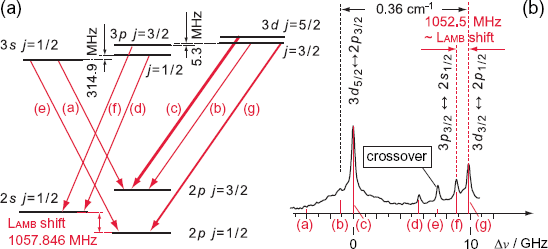
\includegraphics[width=8cm]{src/FineStHyd.png}
    \caption{各谱线的强度分布}
\end{figure}

% subsubsection 氢原子光谱的精细结构 (end)

\subsubsection{Lamb移位} % (fold)
\label{ssub:lamb移位}

精密测量的双线间隔比理论值小了$\SI{0.010}{\per\centi\meter}$. 这是由于$\ce{^2S_{1/2}}$的能级比$\ce{^2P_{1/2}}$高了$\SI{0.03}{\per\centi\meter}$.

\begin{figure}[ht]
    \centering
    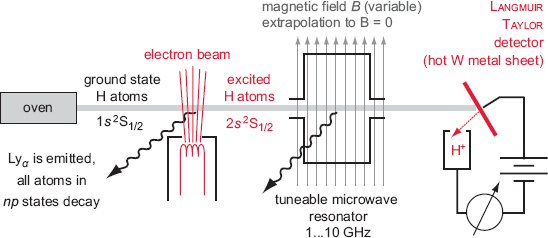
\includegraphics[width=8cm]{src/LambApp.png}
    \caption{Lamb移位测量}
\end{figure}

将氢分子热解离, 得到氢原子, 经过小孔后得到氢原子束, 利用电子轰击以制造$\ce{^2S_{1/2}}$和$\ce{^2P_{1/2}}$态. 由于选择定则, $\ce{^2S_{1/2}}$是亚稳态. 撞击脱出功为$\SI{4.52}{\eV}$的钨. 通过调整磁场的共振频率使$\ce{^2S_{1/2}}$被激发到$\ce{^2P_{1/2}}$或$\ce{^2P_{3/2}}$, 可退去亚稳态, 不再令钨电离. 共振频率调至$\SI{1058}{\mega\hertz}$时可观察到此种现象, 此为Lamb移位之频率.
\begin{cenum}
    \item 不同的能级都存在Lamb移位.
    \item $j=1/2$的Lamb移位最大, $j>1/2$的可忽略.
    \item $n$越大, Lamb移位越小.
\end{cenum}
\begin{remark}[物理图像]
    在量子力学中, 真空亦包含稍纵即逝的电磁辐射和粒子. 真空中存在快速产生的虚正负电子对, 原子核导致真空极化. 由于极化电荷的存在, 质子的电场受到屏蔽, 其有效电荷数较原有值小. 距离越小, 有效电荷越大. $\ce{^2S_{1/2}}$较$\ce{^2P_{1/2}}$电子为近, 感受到的有效电荷较大, 故修正能级的位置相对较低. 这导致氢原子的$\ce{^2P_{1/2}}$降低$\SI{27}{\mega\hertz}$.
    \par
    此外还需要考虑电子的自能修正, 即真空中的虚光子导致零场强的起伏, 其平均值虽为零, 均方值非零. 场强起伏导致电子轨道随机抖动, 产生微小变化
    \[ \expc{\Delta E} = -\frac{e^2}{4\pi\epsilon_0}\expc{\rec{r+\delta r}}. \]
    这贡献了$+\SI{1017}{\mega\eV}$的位移.
    \par
    电子的反常磁矩为
    \[ \abs{\mu_{sz}} \approx \pare{1.00119 \pm 0.00005}\mu_B. \]
    令$g_s = 2\pare{1+a}$, 则
    \[ a_{ex} = \SI{1159652188.4e-12}{}. \]
    这贡献了$+\SI{68}{\mega\hertz}$的位移.
\end{remark}

% subsubsection lamb移位 (end)

\subsubsection{超精细结构} % (fold)
\label{ssub:超精细结构}

原子核并非质点, 而是具有自旋角动量和相应的自旋磁矩. 每个核子都有内禀角动量, 自旋$\displaystyle \half$. 核子在原子核内运动也有相应的轨道角动量. 这产生了总的基态角动量$\+vI$, 满足
\[ \+vI^2 = I\pare{I+1}\hbar^2. \]
$I$是核自旋角动量量子数. 自旋角动量为$\+vI$的带正电荷的原子核具有相应的磁矩
\[ \+v\mu_I = g_I \mu\+_N_ \frac{\+vI}{\hbar}. \]
其中$\displaystyle \mu\+_N_ = \frac{e\hbar}{2M_p}$是\gloss{核磁子}. 显然$\mu_N/\mu_B \approx 1/1837$. $g_I$是回磁比.
\par
此外, 原子核还具有电四极矩.
\[ D = \rec{e}\int \rho\pare{3z'^2 - r'^2}\,\rd{V'} = \frac{2}{5}Z\pare{c^2 - a^2}, \]
其中对称轴方向半轴为$c$, 垂直于对称轴的两个半轴为$a$. 这对电势贡献修正
\[ \varphi = \frac{ZeD}{4\pi\epsilon_0 r^3}. \]
原子核磁矩在电子运动产生的磁场中的取向势能为
\[ \Delta E = -\+v\mu_l\cdot \+vB_e. \]
电四极矩在核外电子分布于原子核处存在梯度时会引发能量移动. 但
\begin{cenum}
    \item 对于$I=0$和$\displaystyle I = \half$的情形, 电四极矩为零.
    \item  对于电子总角动量$J = 0$或$\displaystyle J = \half$的原子, 其在核外电子处产生的电场梯度为零.
\end{cenum}
两种情形皆不发生电四极矩相互作用.
\begin{ex}
    铯原子基态$\ce{^2S_{1/2}}$, $J=1/2$, 核自旋$7/2$, 此时无电四极矩相互作用.
\end{ex}
这些相互作用对能级的影响比精细结构少两到三个数量级, 引入了\gloss{超精细结构}.

% subsubsection 超精细结构 (end)

\subsubsection{原子核自旋和电子运动的相互作用} % (fold)
\label{ssub:原子核自旋和电子运动的相互作用}

核磁矩$\+v\mu_I = g_I \mu\+_N_\+vI/\hbar$, $\+vB_e \propto \+vJ$,
\[ \Delta E = A\+vI\cdot \+vJ. \]
其中$A$谓超精细相互作用常数. 引入原子体系的总角动量$\+vF$, 则
\begin{align*}
    \+vF &= \+vI + \+vJ,\quad \+vF^2 = F\pare{F+1}\hbar,\quad F_z = m_F \hbar, \\
    F &= \pare{I+J},\cdots,\abs{I-J},\quad M_F = -F,-F+1,\cdots,F-1,F.
\end{align*}
可以得到
\[ \+vI\cdot \+vJ = \half\brac{\+vF^2 - \+vI^2 - \+vJ^2} = \frac{\hbar^2}{2}\brac{F\pare{F+1} - J\pare{J+1} - I\pare{I+1}}. \]
代入$\Delta E = A \+vI\cdot \+vJ$, 有
\[ \resumath{\Delta E = \frac{a}{2}\brac{F\pare{F+1} - J\pare{J+1} - I\pare{I+1}}.} \]
对于类氢原子, 可得
\[ a = -2g_I \pare{\frac{m_e}{M_p}}\frac{\alpha^2Z}{n}E_n \rec{j\pare{j+1}\pare{2l+1}}. \]
故精细结构相互作用能$\propto \alpha^2 E_n$, 而超精细结构相互作用能$\propto \pare{m_e/M_p}\alpha^2 E_n$.
\begin{center}
    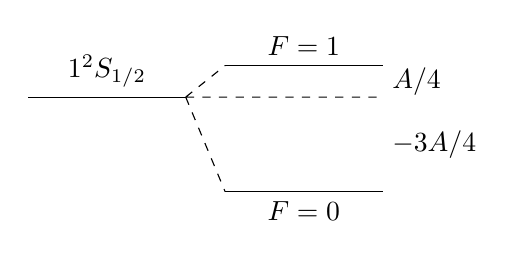
\begin{tikzpicture}
        \draw (-2.5,0) -- (-0.5,0)
        (-1.5,0) node[above] {$\ce{1^2S_{1/2}}$}
        (0,-1.2) -- (2,-1.2)
        (0,0.4)  -- (2,0.4)
        (1,0.4) node[above] {$F=1$}
        (1,-1.2) node[below] {$F=0$}
        (2,0.2) node[right] {$A/4$}
        (2,-0.6) node[right] {$-3A/4$}
        ;
        \draw[dashed] (-0.5,0) -- (0,-1.2) (-0.5,0) --(0,0.4) (-0.5,0) -- (2,0);
    \end{tikzpicture}
\end{center}
\begin{ex}
    对于氢原子的基态$\ce{1^2S_{1/2}}$, $j = 1/2, I = 1/2 \Rightarrow F = 1,0$, 基态能级分裂为两个超精细结构能级, 能量修正分别为
    \[ \Delta = \begin{cases}
        \displaystyle +\rec{4} a, & F=1, \\[.5em]
        \displaystyle -\frac{3}{4} a, & F=0.
    \end{cases} \]
    能级间隔为$a$. 氢原子基态$n=1,l=0,j=1/2,Z=1$的系数$a$的表达式为
    \[ a = \frac{4}{3}g_I\pare{\frac{m_e}{M_p}}m_ec^2\alpha^4. \]
    其中$g_I = \SI{5.58569447}{}$. 这两个超精细结构能级之间的跃迁频率和波长为
    \[ \nu = \SI{1420}{\mega\hertz}, \quad \lambda \approx \SI{21}{\centi\meter}. \]
\end{ex}
超精细结构导致精细结构下简并的固定的$j$分裂为两个能级.
\begin{remark}
    通过向原子束施加共振腔可探测超精细结构的移位.
\end{remark}
\begin{ex}
    铯原子的基态为$\ce{6^2S_{1/2}}$, 核自旋为$7/2$, 基态$j=1/2, I=7/2$, $F=4,3$. 测量得到基态超精细跃迁频率
    \[ \nu = \SI{9192631770}{\hertz}. \]
\end{ex}

% subsubsection 原子核自旋和电子运动的相互作用 (end)

% subsection 氢原子能级的精细结构 (end)

\subsection{碱金属原子} % (fold)
\label{sub:碱金属原子}

\subsubsection{量子数亏损} % (fold)
\label{ssub:量子数亏损}

基态价电子处于$n\ce{s}$态.

\paragraph{隧穿效应} % (fold)
\label{par:隧穿效应}

价电子处于$n\ce{s}$态, 或激发到不同$l$量子数的轨道看到的有效电荷数$Z^*$不同, 且$Z^*>1$. 对应的激发态能级不同程度下降.
\[ E_n = -\half \mu \alpha^2 c^2 \frac{Z^{*2}}{n^2}. \]
由于隧穿效应,
\[ Z^*_{ns} > Z^*_{np} > Z^*_{nd} > \cdots. \]
以及
\[ E_{nl} = -\half \mu\alpha^2 c^2 \frac{Z^*_{nl}}{n^2} = -\half \mu \alpha^2c^2 \rec{n^{*2}}. \]
其中$\displaystyle n^* = n/Z_{nl}^*$. 由于$Z^*_{nl} > 1$, 有$n^* < n$, $n^* = n - \Delta_{n;}$. 其中$\Delta_{nl}$谓量子数亏损.
\[ E_{nl} = -\half \mu\alpha^2c^2 \rec{\pare{n-\Delta_{nl}}^2}. \]
\begin{figure}[ht]
    \centering
    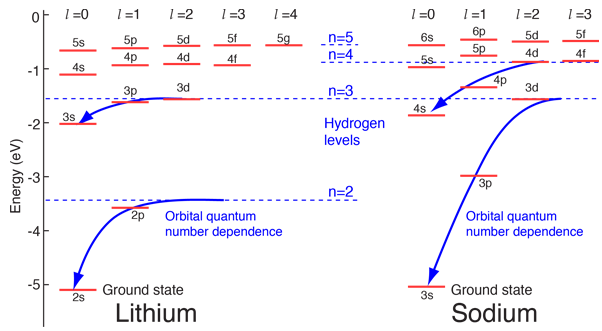
\includegraphics[width=8cm]{src/LevelComp.png}
\end{figure}

% paragraph 隧穿效应 (end)

% subsubsection 量子数亏损 (end)

% subsection 碱金属原子 (end)

% section 电子的自旋和原子能级的精细结构 (end)

\end{document}
